\documentclass{beamer}

%\pgfpagelayout{2 on 1}[a4paper]

\usepackage[T1]{fontenc}
%\usepackage{beamerthemesplit,bm}
\usepackage{graphicx}
% \usepackage{movie15}
\usepackage{hyperref}
\usepackage{multimedia}
\usepackage{subfigure}
\usepackage{xcolor}
\usepackage{amsmath,amssymb}
\usepackage{stmaryrd}

\usetheme{Boadilla}


%\definecolor{mygreen}{rgb}{0,0.48,0.0}

%\definecolor{myblue}{rgb}{0,0,0.64}

\author{Antonio Cervone}
\date{October 12 2012}
\institute{Politecnico di Milano}

\begin{document}

%---------------------------------------------------------------------------------

\begin{frame}

    \frametitle{Gnuplot}

    \begin{block}{Introduction to}
        \centering
        Gnuplot
    \end{block}

    \vspace{1cm}

    \begin{block}{Useful web pages}
        \centering
        \begin{itemize}
            \item http://www.gnuplot.info/
            \item http://t16web.lanl.gov/Kawano/gnuplot/legend-e.html
        \end{itemize}
    \end{block}

\end{frame}

%---------------------------------------------------------------------------------

\begin{frame}

    \frametitle{Gnuplot}

    \begin{block}{Gnuplot}
        \centering
        Gnuplot is a command line utility that is very useful to visualize
        mathematical functions and data in an interactive way.
    \end{block}

    \vspace{1cm}

    \begin{block}{}
        It is used also as visualization toolkit in many applications, such as
        \texttt{octave}.
    \end{block}

\end{frame}

%---------------------------------------------------------------------------------

\begin{frame}

    \frametitle{Gnuplot}

    \begin{block}{Examples}

        \centering
    
        \begin{minipage}{0.5\textwidth}
            \centering
            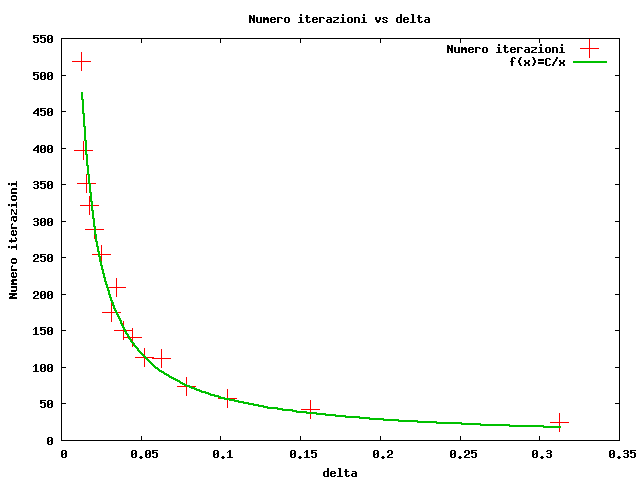
\includegraphics[width=0.95\textwidth]{images/iter_vs_delta}
        \end{minipage}%
        \begin{minipage}{0.5\textwidth}
            \centering
            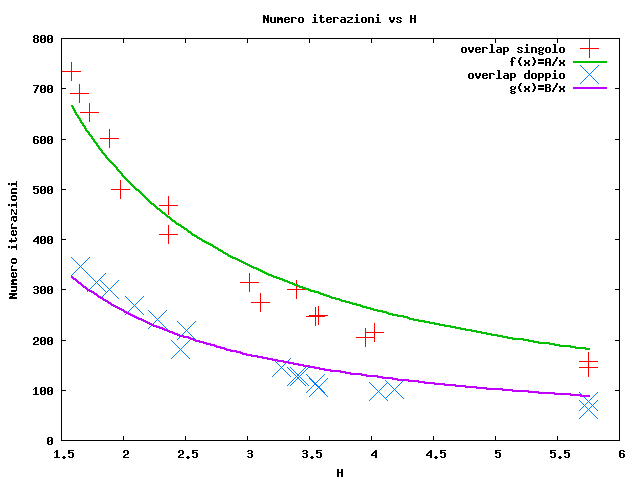
\includegraphics[width=0.95\textwidth]{images/iter_vs_H}
        \end{minipage}

    \end{block}

\end{frame}

%---------------------------------------------------------------------------------

\begin{frame}

    \frametitle{Gnuplot}

    \begin{block}{Examples}

        \centering

        \begin{minipage}{0.5\textwidth}
            \centering
            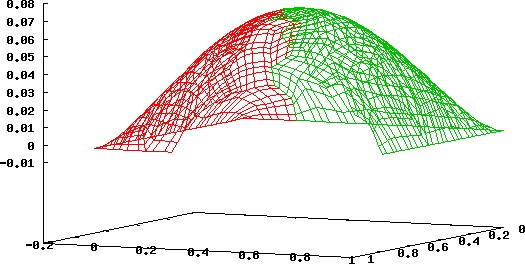
\includegraphics[width=0.95\textwidth]{images/img1}
        \end{minipage}%
        \begin{minipage}{0.5\textwidth}
            \centering
            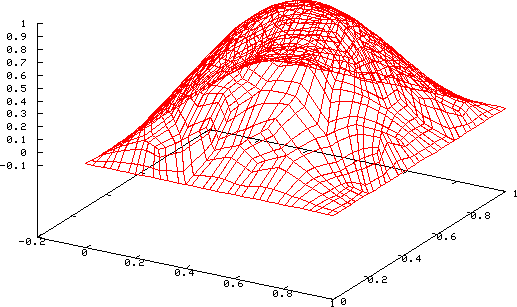
\includegraphics[width=0.95\textwidth]{images/soluzione2}
        \end{minipage}

    \end{block}

\end{frame}

%---------------------------------------------------------------------------------

\begin{frame}[fragile]

    \frametitle{Gnuplot}

    \begin{block}{Commands to plot the last graph}
        \begin{verbatim}
        set terminal png
        set key off
        set output "solution/solution.png"
        splot "solution/solution.dat" with lines
        \end{verbatim}
    \end{block}

    \vspace{1cm}

    \begin{block}{ }
        The biggest problem with gnuplot is saving data correctly for the
        visualization.
    \end{block}

\end{frame}

%---------------------------------------------------------------------------------

\begin{frame}[fragile]

    \frametitle{Gnuplot}

    \begin{block}{Problem}
        Given the \verb1data1 file, visualize the corresponding curves.
    \end{block}
    
    \begin{block}{data}
        \begin{verbatim}
            #   X         Y1         Y2         Y3
   -1.0000    0.0000     0.0000     1.0000
   -0.9000    0.5700     1.1769     0.7150
   -0.8000    1.0800     1.4400     0.4600
   -0.7000    1.5300     1.4997     0.2350
   -0.6000    1.9200     1.4400     0.0400
   -0.5000    2.2500     1.2990    -0.1250
   -0.4000    2.5200     1.0998    -0.2600
   -0.3000    2.7300     0.8585    -0.3650
   -0.2000    2.8800     0.5879    -0.4400
   -0.1000    2.9700     0.2985    -0.4850
    0.0000    3.0000    -0.0000    -0.5000
    0.1000    2.9700    -0.2985    -0.4850
    0.2000    2.8800    -0.5879    -0.4400
    0.3000    2.7300    -0.8585    -0.3650
    0.4000    2.5200    -1.0998    -0.2600
    0.5000    2.2500    -1.2990    -0.1250
    0.6000    1.9200    -1.4400     0.0400
    0.7000    1.5300    -1.4997     0.2350
    0.8000    1.0800    -1.4400     0.4600
    0.9000    0.5700    -1.1769     0.7150
    1.0000    0.0000    -0.0000     1.0000

        \end{verbatim}
    \end{block}

\end{frame}

%---------------------------------------------------------------------------------

\begin{frame}[fragile]

    \frametitle{Gnuplot}

    \begin{block}{Gnuplot commands}
        \begin{verbatim}
            plot "data" using 1:2 with lines,\
                 "data" using 1:3 with lines,\
                 "data" using 1:4 with lines
        \end{verbatim}
    \end{block}

    \begin{center}
        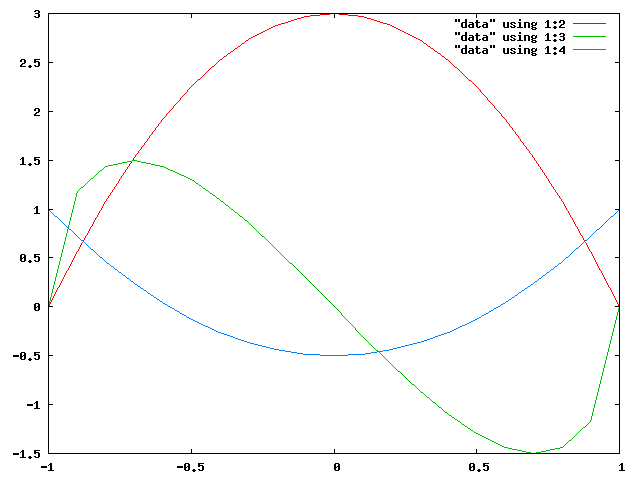
\includegraphics[width=0.5\textwidth]{images/graph}
    \end{center}

\end{frame}

%---------------------------------------------------------------------------------

\begin{frame}[fragile]

    \frametitle{Gnuplot}

    \begin{block}{The commands to set up the output must be given before the
    plot command.}

        \begin{verbatim}
        set terminal png
        set output "graph.png"
        \end{verbatim}

    \end{block}

    \vspace{1cm}

    \begin{block}{}
        Gnuplot supports many output formats: png, fig, pslatex, svg, tikz, \ldots
    \end{block}

    \vspace{1cm}

    \begin{block}{To go back to screen visualization}

        \begin{verbatim}
        set terminal x11
        \end{verbatim}

    \end{block}

\end{frame}

%---------------------------------------------------------------------------------

\begin{frame}[fragile]

    \frametitle{Gnuplot}

    \begin{block}{ }
        Gnuplot can also execute scripts from file.

        \begin{verbatim}
        gnuplot script_file
        \end{verbatim}

    \end{block}

    \vspace{1cm}

    \begin{block}{C++}
        Gnuplot can be invoked from a C++ listing with the \texttt{system} call
        in the \texttt{cstdlib} header.

        \begin{verbatim}
            system("gnuplot script_file");
        \end{verbatim}

        In fact the \texttt{system} command can be used to execute any
        operating system command.
    \end{block}

\end{frame}

\end{document}

